\documentclass{beamer}
\setbeamertemplate{footline}[frame number]

\usepackage[utf8x]{inputenc}
\usepackage[brazil,british]{babel}
\usetheme{default} 
\usecolortheme{beaver}
\newtranslation[to=brazil]{Theorem}{Teorema}
\newtranslation[to=brazil]{Definition}{Definição}
\newtranslation[to=brazil]{Example}{Exemplo}
\newtranslation[to=brazil]{Problem}{Exercício}
\newtranslation[to=brazil]{Solution}{Resolução}
\logo{
\includegraphics[width=1cm]{../img/logo-ppgsc-icon-text.png}}

\usepackage{graphicx}
\usepackage{clrscode3e}
\usepackage{hyperref}

\usepackage{pgf}
\usepackage{tikz}
\newcommand{\assert}[1]{\textcolor{blue}{#1}}



\title{Aula 25: Grafos: árvores geradoras mínimas}
\subtitle{Árvores de extensão mínima}
\author{David Déharbe \\
  Programa de Pós-graduação em Sistemas e Computação \\
  Universidade Federal do Rio Grande do Norte \\
  Centro de Ciências Exatas e da Terra \\
  Departamento de Informática e Matemática Aplicada}
\date{20 de maio de 2015}

\begin{document}
\selectlanguage{brazil}

\begin{frame}
  \titlepage
\end{frame}

\begin{frame}
  \frametitle{Plano}
\begin{center}
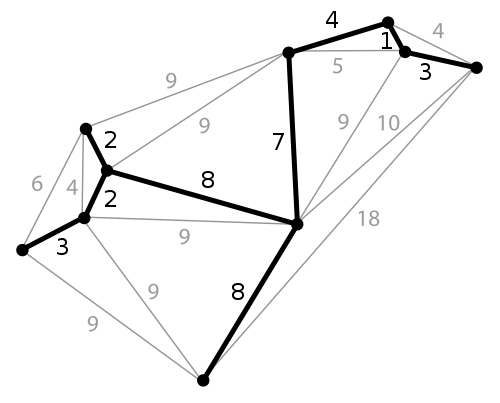
\includegraphics[height=.5\textheight]{fig/minimum_spanning_tree.png}
\end{center}
  \tableofcontents
Referência: Cormen, cap 24.
\end{frame}

\section{Introdução}

\begin{frame}
\frametitle{Introdução}

\begin{itemize}
\item Exemplo
\begin{itemize}
\item rede ótica interligando diferentes institutos
\item $C_{AB}$ custo para conectar instituto $A$ ao instituto $B$
\item identificar qual a rede que minimiza os custos
\end{itemize}
\item \alert{otimização combinatória}: árvore geradora mínima 

\textit{minimum spanning tree}
\end{itemize}

\end{frame}

\begin{frame}
\frametitle{Formalização}

\begin{itemize}
\item entrada: grafo não dirigido com pesos $G = (V, E, w)$
\item saída: $T$ subconjunto acíclico de $E$ tal que
\begin{enumerate}
\item $w(T) = \sum_{e \in T} w(e)$ é o menor possível
\item $T$ connecta todos os elementos de $V$
\end{enumerate}
\item $T$ acíclico $\Rightarrow$ $T$ é uma \alert{árvore}
\item $T$ connecta todos os vértices: é uma \alert{cobertura} de $G$
\item a soma dos pesos das arestas é o \alert{mínimo} possível
\end{itemize}
\end{frame}

\begin{frame}
\frametitle{Abordagem algorítmica}

\begin{itemize}
\item abordagem \alert{gulosa}
\begin{itemize}
\item solução parcial pode ser estendida a uma solução completa
\item a solução é construída incrementalmente
\item uma sequência de decisões localmente ótimas gera uma solução global ótima
\end{itemize}
\item dois algoritmos
\begin{itemize}
\item Vojtech Jarník (1930), Robert \alert{Prim} (1957), Edsger Dijkstra (1959)
\item Joseph \alert{Kruskal} (1956)
\item ambos são casos particulares de um algoritmo abstrato
\end{itemize}
\end{itemize}
\end{frame}

\section{Um algoritmo abstrato}

\begin{frame}
\frametitle{Crescendo uma árvore geradora mínima}
\framesubtitle{Algoritmo abstrato}

\begin{itemize}
\item $A$: sub-conjunto de uma árvore geradora mínima
\begin{itemize}
\item $A$ não pode ter ciclos
\item o grafo induzido por $A$ não precisa ser conectado
\item $A$ forma uma floresta de árvores
\end{itemize}
\item iterativamente uma aresta $(u, v)$ é adicionada a $A$
\begin{itemize}
\item $(u, v)$ é \alert{segura} se $A \cup \{(u, v)\}$ é um sub-conjunto de uma árvore geradora mínima.
\end{itemize}
\item $A$ continua um sub-conjunto de uma árvore geradora mínima
\item término: $A$ cobre todo o grafo
\end{itemize}
\end{frame}

\begin{frame}
\frametitle{Crescendo uma árvore geradora mínima}
\framesubtitle{Algoritmo abstrato}

\begin{itemize}
\item $A$: sub-conjunto de uma árvore geradora mínima
\item iterativamente uma aresta $(u, v)$ é adicionada a $A$
\begin{itemize}
\item $(u, v)$ é \alert{segura} se $A \cup \{(u, v)\}$ é uma árvore geradora mínima.
\end{itemize}
\item $A$ continua um sub-conjunto de uma árvore geradora mínima
\item término: $A$ cobre todo o grafo
\end{itemize}
\end{frame}

\begin{frame}
\frametitle{Crescendo uma árvore geradora mínima}
\framesubtitle{Algoritmo abstrato}

\begin{codebox}
\Procname{$\proc{MST-Abstract}(G)$}
\zi $A \gets \emptyset$
\zi \assert{\Comment invariante: $A \subseteq$ uma árvore geradora mínima}
\zi \While $A$ não forma uma árvore geradora mínima
\zi \Do Escolher uma aresta $(u, v)$ segura para $A$
\zi   $A \gets A \cup \{ (u, v) \}$
    \End
\zi \Return $A$
\end{codebox}
\pause
\alert{Questão:} Como identificar uma aresta segura para $A$?
\end{frame}

\begin{frame}
\frametitle{Identificação de aresta segura}
\framesubtitle{Roteiro}

\begin{itemize}
\item Definições:
\begin{itemize}
\item corte de um grafo não dirigido
\item aresta leve
\end{itemize}
\item Propriedades
\begin{itemize}
\item teorema: arestas leves e subconjunto de árvores geradora mínima
\item corolário (fundamentação dos algoritmos de Prim e Kruskal):
  componentes conectados e arestas leves.
\end{itemize}
\end{itemize}
\end{frame}

\begin{frame}
\frametitle{Definições}

\begin{definition}[Corte]
Seja $G=(V, E)$ um grafo não dirigido. Um \alert{corte} de $G$ é uma
partição $(S, V - S)$ dos vértices.
\end{definition}

\begin{definition}
Seja $G=(V, E)$ um grafo não dirigido e $(S, V - S)$ um corte de
$G$. 
\begin{itemize}
\item A aresta $(u, v)$ \alert{cruza} o corte se $u \in S$ e $v \in
  V-S$.
\item O conjunto de arestas $A \subseteq E$ \alert{respeita} o corte
  se nenhuma aresta de $A$ cruza o corte.
\item Se $G$ é um grafo com pesos, a aresta $(u, v) \in E$ é uma
  \alert{aresta leve} se atravessa o corte e tem o menor peso entre
  todas as arestas cruzando o corte.
\end{itemize}
\end{definition}

\end{frame}

\begin{frame}
\frametitle{Definições}
\framesubtitle{Ilustração}

\begin{center}
\includegraphics[width=.9\textwidth]{fig/mst-2.pdf}
\end{center}

\begin{itemize}
\item corte, aresta cruzando corte, aresta leve, conjunto de arestas
respeitando o corte
\end{itemize}

\end{frame}

\begin{frame}
\frametitle{Propriedades}
\framesubtitle{Teorema}

O teorema seguinte fornece um critério para escolher arestas
no algoritmo abstrato:
\begin{theorem}[Critério da arestas leve]
Seja $G = (V, E, w)$ um grafo não dirigido conectado com pesos. 
Seja $A \subseteq E$, tal que $A$ é um sub-conjunto de uma árvore de
cobertura mínima. Seja $(S, V-S)$ um corte que respeita $A$, e $(u, v)$
uma aresta leve cruzando $(S, V-S)$. Então $(u, v)$ é seguro para $A$.
\end{theorem}
\end{frame}

\begin{frame}
\frametitle{O teorema em ação}

\begin{center}
\includegraphics[width=.9\textwidth]{fig/mst-2.pdf}
\end{center}

\begin{center}
\includegraphics[width=.9\textwidth]{fig/mst-3.pdf}
\end{center}

\end{frame}

\begin{frame}
\frametitle{Pratique}
\begin{center}
\includegraphics[height=.4\textheight]{fig/mst-1.pdf}
\end{center}
\begin{codebox}
\zi $A \gets \emptyset$
\zi \While $A$ não forma uma árvore geradora mínima
\zi \Do Escolher uma aresta $(u, v)$ segura para $A$
\zi   $A \gets A \cup \{ (u, v) \}$
    \End
\end{codebox}

$(u, v)$ é seguro para $A$:
\begin{itemize}
\item $A$ é um sub-conjunto de uma árvore geradora mínima. 
\item $(S, V-S)$ respeita $A$, 
\item $(u, v)$ uma aresta leve cruzando $(S, V-S)$. 
\end{itemize}

\end{frame}

\begin{frame}
\frametitle{Demonstração}
\framesubtitle{Teorema}

\only<1-2>{
\begin{theorem}[Critério da arestas leve]
Seja $G = (V, E, w)$ um grafo não dirigido conectado com pesos. 
Seja $A \subseteq E$, tal que $A$ é um sub-conjunto de uma árvore de
cobertura mínima. Seja $(S, V-S)$ um corte que respeita $A$, e $(u, v)$
uma aresta leve cruzando $(S, V-S)$. Então $(u, v)$ é seguro para $A$.
\end{theorem}
}
\only<2->{
\begin{small}
\begin{proof}
\begin{itemize}
\only<2>{
\item hipótese 1: $A \subseteq T$, $T$ é uma árvore geradora mínima
\item conclusão: $\exists T' \cdot A \cup \{(u, v)\} \subseteq T'$, $T'$ árvore geradora mínima
\item Duas possibilidades
\begin{enumerate}
\item Se $(u, v) \in T$, então $T' = T$
\item Se $(u, v) \not\in T$, vamos construir $T'$
\end{enumerate}
}
\only<3>{
\item $A \subseteq T$, $T$ é uma árvore geradora mínima, $(u, v) \not\in T$,
\item hipótese 2: $(u, v)$ cruza $(S, V-S)$.
\begin{center}
\includegraphics[height=.5\textheight]{fig/mst-4.pdf}
\end{center}
}
\only<4>{
\item em $T$, $u \leadsto v$, seja $p$ o caminho:  $p, (u, v)$ formam um ciclo
\begin{center}
\includegraphics[height=.5\textheight]{fig/mst-5.pdf}
\end{center}
}
\only<5->{
\only<5>{
\item existe $(x, y) \in p$ tal que $(x, y)$ cruza $(S, V-S)$.
\item hipótese 3: $A$ respeita $(S, V-S)$, logo $(x, y) \not\in A$.
}
\only<6>{
\item $T - \{(x, y)\}$ resulta em duas árvores não conexas
\item $T'= (T - \{(x, y)\}) \cup \{(u, v)\}$ é uma árvore geradora
}
\only<7>{
\item hipótese 4: $(u, v)$ é uma aresta leve
\item logo $w(u, v) \le w(x, y)$, e $w(T') \le w(T)$: $T'$ é árvore geradora mínima.
}
\begin{center}
\includegraphics[height=.5\textheight]{fig/mst-6.pdf}
\end{center}
}
\end{itemize}
\end{proof}
\end{small}
}
\end{frame}

\begin{frame}
\frametitle{Propriedades}
\framesubtitle{Corolário}

\begin{corollary}
Seja $G = (V, E, w)$ um grafo não dirigido conectado com pesos. 
Seja $A \subseteq E$, tal que $A$ é um sub-conjunto de uma árvore de
cobertura mínima. Seja $C$ uma árvore na floresta $G_A = (V, A)$,

Se $(u, v)$ é uma aresta leve conectando $C$ a uma outra árvore
de $G_A$, então $(u, v)$ é segura para $A$.
\end{corollary}

\begin{proof}
\begin{itemize}
\item Por definição, $(C, V-C)$ é um corte que respeita $A$. 
\item A aresta $(u, v)$ é uma aresta leve cruzando $(C, V-C)$
\item O teorema diz que $(u, v)$ é uma aresta segura para $A$.
\end{itemize}
\end{proof}
\end{frame}

\section{Algoritmo de Kruskal}

\begin{frame}
\frametitle{Algoritmo de Kruskal}
\framesubtitle{Princípios}

\begin{itemize}
\item instancia o algoritmo abstrato
\item mantem uma floresta de sub-conjuntos de árvore geradora mínima
\begin{itemize}
\item inicialmente cada vértice forma uma árvore individualmente
\end{itemize}
\item abordagem gulosa: escolha a menor aresta que connecta duas árvores
  da floresta
\begin{itemize}
\item decrementa o número de árvores na floresta
\end{itemize}
\item término: a floresta tem uma árvore, geradora mínima
\item \alert{abordagem gulosa} (\textit{greedy\/})
\end{itemize}

\end{frame}

\begin{frame}
\frametitle{Algoritmo de Kruskal}

\begin{codebox}
\Procname{$\proc{MST-Kruskal}(G)$} 
\li $A \gets \emptyset$
\li \For $v \in \attrib{G}{V}$
\li \Do $\proc{Make-Set}(v)$
    \End
\li Ordena $\attrib{G}{E}$ por peso crescente
\li \For $(u, v) \in \attrib{G}{E}$, em ordem crescente de peso
\li \Do \If $\proc{Find-Set}(u) \neq \proc{Find-Set}(v)$
\li   \Then $A \gets A \cup \{ (u, v) \}$
\li     $\proc{Union}(u, v)$
      \End
    \End
\end{codebox}

\end{frame}

\begin{frame}
\frametitle{Algoritmo de Kruskal}
\framesubtitle{Pratique}

\begin{center}
\includegraphics[width=\textwidth]{fig/mst-1.pdf}
\end{center}

\end{frame}

\begin{frame}
\frametitle{Algoritmo de Kruskal}
\framesubtitle{Complexidade}

\begin{itemize}
\item Estrutura de dados:
\begin{itemize}
\item conjuntos disjuntos com união por tamanho e compressão de caminho
\item melhor complexidade assintótica conhecida
\end{itemize}
\item Inicialização: $\Theta(V)$
\item Ordenação das arestas: $O(E \lg E)$
\item $\Theta(E)$ operações sobre florestas de árvore: $O(E \lg E)$
\item Grafo conectado $E \in \Omega(V), E \in O(V^2)$
\item Total: $O(E \lg E)$
\end{itemize}

\end{frame}

\section{Algoritmo de Prim}

\begin{frame}
\frametitle{Algoritmo de Prim}
\framesubtitle{Princípios}

\begin{itemize}
\item $A$ forma uma (única) árvore
\item a cada iteração uma aresta segura é adicionada a $A$
\item a aresta acrescentado é aquela que soma o menor peso
\item abordagem gulosa
\item ponto principal: como identificar eficazmente a aresta que soma o menor peso
\begin{itemize}
\item fila de prioridade dos vértices que não estão em $A$
\item prioridade de $v$: $\attrib{v}{key}$ menor distância do vértice até um vértice de $A$
\item $\attrib{v}{up}$ vértice de $A$ ao qual o $v$ é conectado quando
  $(v,\attrib{v}{up})$ é acrescentado a $A$.
\end{itemize}
\end{itemize}

\end{frame}

\begin{frame}
\frametitle{Algoritmo de Prim}

\begin{codebox}
\Procname{$\proc{MST-Prim}(G)$}
\li selecionar $r \in V$ qualquer
\li \For $u \in \attrib{G}{V}$
\li \Do $\attrib{u}{key} \gets \infty$
    \End
\li $\attrib{r}{key} \gets 0$
\li $\attrib{r}{up} \gets \const{Nil}$
\li $Q \gets \attrib{G}{V}$
\li \While $Q \neq \emptyset$
\li \Do $u \gets \proc{Extract-Min}(Q)$
\li   \For $v \in \attrib{u}{adj}$
\li   \Do \If $v \in Q$ e $w(u, v) < \attrib{v}{key}$
\li     \Then $\attrib{v}{up} \gets u$
\li       $\attrib{v}{key} \gets w(u, v)$
        \End
      \End
    \End
\end{codebox}

\end{frame}

\begin{frame}
\frametitle{Ilustração}
\framesubtitle{Algoritmo de Prim}

\begin{center}
\includegraphics[width=\textwidth]{fig/mst-1.pdf}
\end{center}

\end{frame}

\begin{frame}
\frametitle{Complexidade}
\framesubtitle{Algoritmo de Prim}

\begin{codebox}
\Procname{$\proc{MST-Prim}(G)$}
\li selecionar $r \in V$ qualquer
\li \For $u \in \attrib{G}{V}$ \assert{\Comment $\Theta(V)$}
\li \Do $\attrib{u}{key} \gets \infty$
    \End
\li $\attrib{r}{key} \gets 0$
\li $\attrib{r}{up} \gets \const{Nil}$
\li $Q \gets \attrib{G}{V}$   \assert{\Comment $O(V)$}
\li \While $Q \neq \emptyset$ \assert{\Comment $\Theta(V)$ vezes}
\li \Do $u \gets \proc{Extract-Min}(Q)$ \assert{\Comment $O(\lg V)$}
\li   \For $v \in \attrib{u}{adj}$ \assert{\Comment total: $\Theta(E)$}
\li   \Do \If $v \in Q$ e $w(u, v) < \attrib{v}{key}$ 
\li     \Then $\attrib{v}{up} \gets u$ \assert{\Comment $O(\lg v)$}
\li       $\attrib{v}{key} \gets w(u, v)$  \assert{\Comment $O(\lg v)$}
        \End
      \End
    \End
\end{codebox}
\pause $O(E \lg V + V \lg V) = O(E \lg V)$
\end{frame}

\end{document}

